% !TeX spellcheck = cs_CZ
\begin{example}\label{TEO:exam005} \textbf{Transformátor}: \newline
  Na primární vinutí vzduchového transformátoru s činitelem $k < 1$ je v čase $t=0$ připojen zdroj 
  napětí $U_1 = konst$. Formulujte postup pro výpočet odezev $i_1(t)$ a $i_2(t)$ pro obecné 
  parametry zapojení a výsledky ověřte simulací pro následující hodnoty: $U_1 = 1V, R_1 = 1\Omega, 
  R_2 = 4\Omega, $ transformátor má převod $1:3$.
  
  {\centering
   \captionsetup{type=figure}
   \includegraphics[width=0.9\linewidth]{Ideal_Trf_step_response_LTspice.pdf}
   \captionof{figure}{\texttt{Transformer.asc}: Zapojení vzduchového transformátoru
              pro simulaci v programu LTSpice}
   \label{TEO:fig_trafo_int_uprim}
   \par}
  
  \textbf{Klasické řešení}: Podle II. Kirchhoffova zákona platí soustava rovnic:
  \begin{subequations}\label{TEO:eq_trafo_IIKz}
    \begin{align}
      R_1i_1 + L_1\frac{di_1}{dt} + L_{12}\frac{di_2}{dt} &= U_1 \\
      R_2i_2 + L_2\frac{di_2}{dt} + L_{12}\frac{di_1}{dt} &= 0
    \end{align}
  \end{subequations}
  
  \begin{equation}\label{TEO:eq_char_rce}
  \left(
  \begin{array}{cc}
  R_1 + L_1\lambda & L_{12}\lambda  \\
  L_{12}\lambda    & R_2 + L_2\lambda
  \end{array}
  \right) = 0
  \end{equation}
  \begin{subequations}\label{TEO:eq_char_rce_solve}
    \begin{align}
      (R_1 + L_1\lambda) - L_{12}^2\lambda^2                                      &= 0      \\
      R_1R_2 + (L_1R_2 + L_2R_1)\lambda + L_1L_2\lambda - L_{12}^2\lambda^2       &= 0      \\
      \lambda^2(L_1L_2-L_{12}^2)+(L_1R_2+L_2R_1)\lambda +R_1R_2                   &= L_1L_2 \\
      \lambda^2(\frac{L_1L_2-L_{12}^2}{L_1L_2})+
      (\frac{L_1R_2+L_2R_1}{L_1L_2})\lambda +\frac{R1R2}{L_1L_2}                  &= 0
    \end{align}
  \end{subequations}
  Zavedeme-li $\tau_1 = \frac{L_1}{R_1}, \tau_2 = \frac{L_2}{R_2}$,
  $k=\frac{L_12}{\sqrt{L_1L_2}}, k^2=\frac{L_12^2}{L_1L_2}$, $\sigma = 1-k^2$ dostaneme
  \begin{subequations}\label{TEO:eq_trafo_vysl_rce}
    \begin{align}
      \sigma\lambda^2 + \left(\frac{1}{\tau_1}+\frac{1}{\tau_2}\right)\lambda + 
      \frac{1}{\tau_1}\frac{1}{\tau_2} = 0                                                 \\
      \lambda^2 + \frac{1}{\sigma}\left(\frac{1}{\tau_1}+\frac{1}{\tau_2}\right)\lambda + 
      \frac{1}{\sigma\tau_1\tau_2} = 0
    \end{align}
  \end{subequations}
  Je-li $\lambda_1 = -\beta+\alpha$ a $\lambda_2 = -\beta-\alpha$
  \begin{subequations}
    \label{TEO:eq_trafo_alphabeta}
    \begin{align}
    \alpha &= \frac{1}{2\sigma}
    \left(\frac{1}{\tau_1}+ 
    \frac{1}{\tau_2}\right)            \label{TEO:eq_trafo_alphabeta_a}     \\ 
    \beta  &= \frac{1}{2\sigma}
    \sqrt{\left(\frac{1}{\tau_1}+
      \frac{1}{\tau_2}\right)^2+
      \frac{4\sigma}{\tau_1\tau_2}}      \label{TEO:eq_trafo_alphabeta_b}
    \end{align}
  \end{subequations}
  Jelikož $k<1$; je $0<\sigma<1$; rozborem rovnice \ref{TEO:eq_trafo_alphabeta_b} plyne, že pak
  je $\alpha\neq0$, reálné. Soustava rovnic \ref{TEO:eq_trafo_IIKz} má tedy obecné řešení
  \begin{subequations}\label{TEO:eq_trafo_obecne_res}
    \begin{align}
      i_1(t) &= i_{1o} +i_{1p} = K_1e^{\lambda_1t} + K_2e^{\lambda_2t} +\frac{U_0}{R} \\
      i_2(t) &= i_{2o} +i_{2p} = K_3e^{\lambda_1t} + K_4e^{\lambda_2t}
    \end{align}
  \end{subequations}
  Integrační konstanty $K_1, K_2, K_3$ a $K_4$ určíme z matematických počátečních podmínek:
  $i_1(0)=i_2(0)=0$ (což jsou zároveň fyzikální počáteční podmínky) a $\frac{di_1}{dt}|_{t=0}, 
  \frac{di_2}{dt}|_{t=0}$, které určíme z rovnic \ref{TEO:eq_trafo_IIKz} pro $t=0$:
  \begin{subequations}\label{TEO:eq_trafo_didt_t0}
    \begin{align}
      L_1i_1'+L_{12}i_2' &= U_0 \Longrightarrow i_1' = \left(\frac{U_0-L_{12}i_2'}{L_1}\right)\\
      L_2i_2'+L_{12}i_1' &= 0
    \end{align}
  \end{subequations}
  Dále postupujeme tak, že do druhé rovnice dosadíme vyjádřenou první derivaci primárního
  proudu z první rovnice a získáme vztah pro první derivaci sekundárního proudu v čase $t=0$:
    \begin{subequations}\label{TEO:eq_trafo_dev_i1i2}
    \begin{align}
      \frac{di_1}{dt}|_{t=0} &=   \frac{L_{2}}{L_1L_2-L_{12}^2}U_0                        \\
      \frac{di_2}{dt}|_{t=0} &=  -\frac{L_{12}}{L_1L_2-L_{12}^2}U_0
    \end{align}
  \end{subequations}
  Aplikací těchto počátečních podmínek na obecné řešení \ref{TEO:eq_trafo_obecne_res} plynou
  vztahy
  \begin{subequations}
    \begin{align}
    i_1(0)                            &= K_1 + K_2 +\frac{U_0}{R}                         \\
    \frac{L_{2}}{L_1L_2-L_{12}^2}U_0  &= \lambda_1K_1 + \lambda_2K_2                      \\
    i_2(0)                            &= K_3 + K_4                                        \\
   -\frac{L_{12}}{L_1L_2-L_{12}^2}U_0 &= \lambda_1K_3 + \lambda_2K_4
    \end{align}
  \end{subequations}
  Z první a třetí rovnice vypočítáme $K_1; K_2$, ze druhé a čtvrté rovnice $K_3; K_4$.
  Do\-sa\-ze\-ním do rovnice \ref{TEO:eq_trafo_obecne_res} dostaneme po úpravě odezvy $i_1(t)$
  a $i_2(t)$. Speciálně pro $R_1=R_2=R$;$L_1=L_2=L$ je
  \begin{subequations}\label{TEO:eq_trafo_solved_RL}
    \begin{align}
      i_1(t) &= \frac{U_0}{2R}\left(2-e^{-\frac{t}{\tau_3}}-e^{-\frac{t}{\tau_4}}\right) \\
      i_2(t) &= \frac{U_0}{2R}\left(-e^{-\frac{t}{\tau_3}}+e^{-\frac{t}{\tau_4}}\right)
    \end{align}
  \end{subequations}
  kde je $\tau_3 = \frac{L + L_{12}}{R}; \tau_4 = \frac{L - L_{12}}{R}$
  
  \textbf{Operátorové řešení}: Laplaceovou transformací rovnice \ref{TEO:eq_trafo_IIKz}
  dostáváme
  \begin{subequations}\label{TEO:eq_trafo_laplace}
    \begin{align}
      (R_1 + pL_1)I_1(p)+pL_{12}I_2(p)   &= \frac{U_0}{p} \\
      pL_{12}I_1(p) + (R_2 + pL_2)I_2(p) &= 0
    \end{align}
  \end{subequations}
  Zavedeme $\sigma; \tau_1; \tau_2$, vypočítáme obrazy proudů a jejich zpětnou transformací
  do\-sta\-ne\-me rovnice pro odezvy $i_1(t)$ a $i_2(t)$.
  
  {\centering
   \captionsetup{type=figure}
   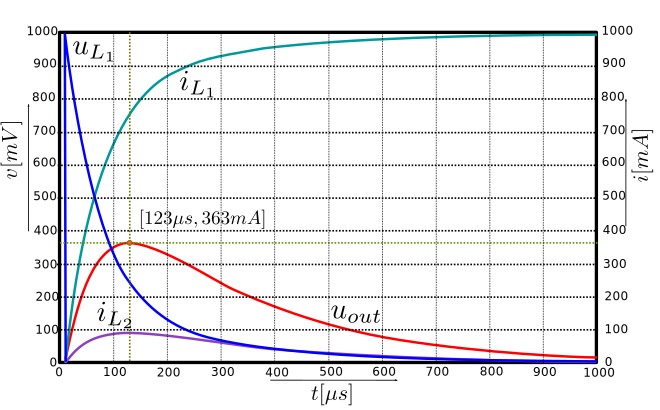
\includegraphics[width=1\linewidth]{Ideal_Trf_step_response_K05.pdf}
   \captionof{figure}{Odezva na jednotkový skok transformátoru s parametry: $k=0.5, L_1 = 100 \mu 
             H, L_2 = 900 \mu H$}
  \label{figure:trafo_int_uprim}
  \par}
\end{example}

